\documentclass[a5paper]{tufte-book}

\usepackage[caption=false]{subfig}
\usepackage{url}
\usepackage{graphicx}

% This document is intended to be read by 8 to 10 year old students.  Edits to
% the language should keep this in mind.

\title{Stop Motion}
\author{}
\date{}

\begin{document}
\maketitle

\section*{Go, go, technology!}

Let's make a movie! You can write it, direct it and film it.  All the equipment is here.  You only need a tablet computer~\ref{fig:tablet} and your imagination.  Our movie making technique is called  \textit{stop motion}.  Using stop motion we create a scene and take a picture of it.  We then make small movements in the scene and take another picture.  If we take enough pictures we can switch between them at high speed.  This fools your brain into thinking that it is seeing movement.

A normal scene in a big-screen movie contains 24 pictures every second.  We're going to create 4 pictures for every second.  This means the movement in your movie will appear to be a little jerky.  This is a limitation of our technology.  Great creators take these limitations and turn them into strengths.  An example stop motion movie can be seen  \href{http://youtu.be/c_13_xEB7sw}{on youtube}\marginnote{\url{http://youtu.be/c_13_xEB7sw}}.  To help you create scenes there are some props.  These include modelling clay, building blocks, some toys and some colours.

\begin{figure}
  \subfloat[]{
    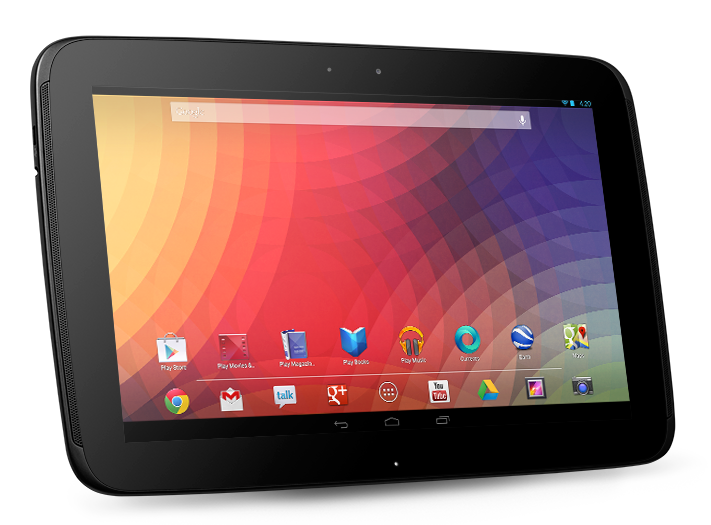
\includegraphics[width=\textwidth]{images/Nexus_10}
    \caption{A tablet computer}
    \label{fig:tablet}
  }
\end{figure}

\section*{Get Fused}

Now we can use the basic software and publish a video, we need to think about the story.  Most movies tell a story.  The story of a movie is called its \textit{plot}.  People have been developing plots for at least 3000 years.  In ancient Greece, Aristotle said that every plot must have a beginning, a middle and an end.  The beginning of a plot is the \textit{setup}, the middle is the \textit{complication} and the end is the \textit{resolution}.  You can think of most movies in these terms.

As an example, the in the story of ``Alice's Adventures in Wonderland''\marginnote{The author of this story used to take his holidays in Eastbourne.} the setup leads Alice from the real world into an imaginary world.  In the complication we find Alice at the Mad Hatter's tea party and playing croquet with the Queen of Hearts who eventually wants to chop Alice's head off!  Alice's sister resolves all the problems in the resolution of the story.

To develop the plot for your movie you may wish to use a \textit{storyboard}.  An example storyboard can be seen in figure~\ref{fig:storyboard}\footnote{Storyboard image by flikr user tmray02 used under \href{http://creativecommons.org/licenses/by-sa/3.0/deed.en}{CC By SA} licence}.  This example storyboard is not neat.  It doesn't need to be.  You use it to sketch ideas and organise them.

\begin{figure}
  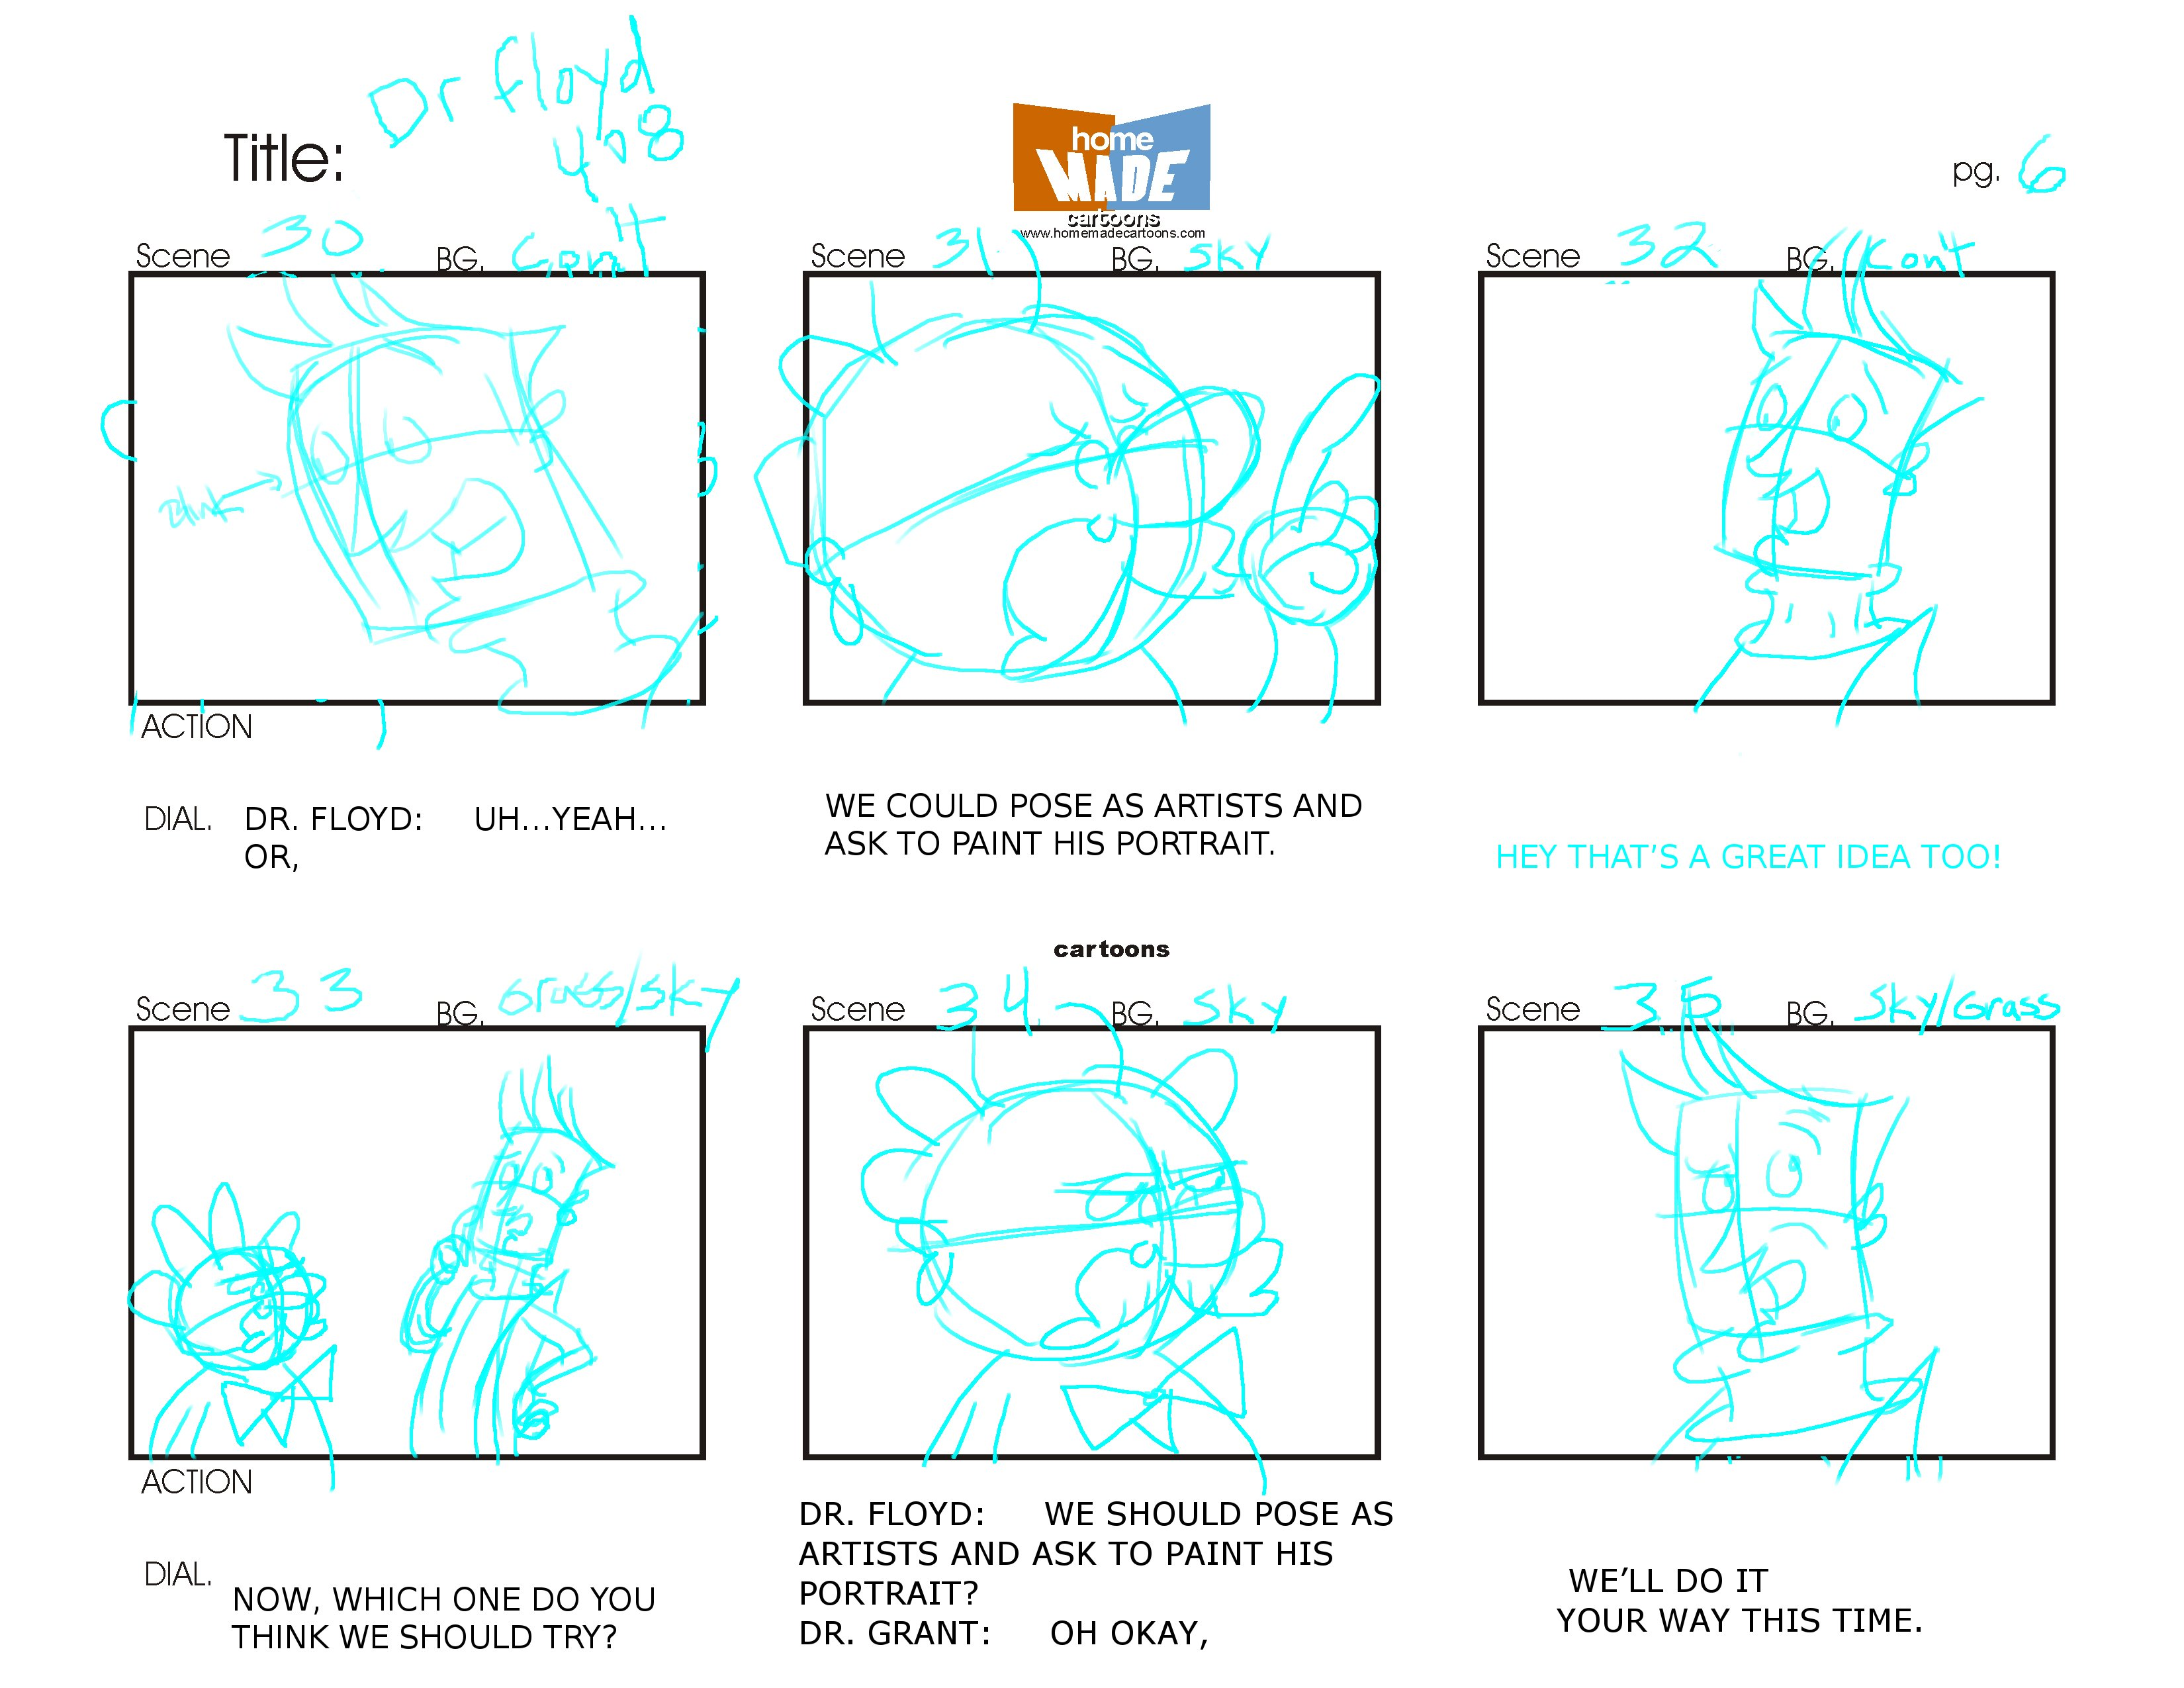
\includegraphics[width=\textwidth]{images/Storyboard_for_The_Radio_Adventures_of_Dr_Floyd}
  \caption{A storyboard}
  \label{fig:storyboard}
\end{figure}

\section*{Super Fused}
Everything can be made better.  How could you make your movie better?  Do you need extra props?  Is the tablet software limiting your creative skills?  How would you make the tablet software better?  Let's make a paper prototype\marginnote{A \textit{paper prototype} is a drawing of how the software should look on the screen.} that explains your improvements.  Have a look at figure~\ref{fig:paper-prototype} for an example of a paper prototype.

The word ``prototype'' is used again and again in software development.  We can make paper prototypes or even a prototype application.  In each case we improve the prototype to make another prototype.  We then improve the improved prototype.  We stop making improvements when the software does what we need it to do and our users are happy with it.  In many cases this process never finishes.  For example, the Firefox web browser has been in development since 1993\marginnote{For interested readers, \href{http://www.mozilla.org/en-GB/firefox/}{Firefox}, is based on \href{http://en.wikipedia.org/wiki/Netscape_Navigator}{Netscape Navigator} which was originally based on \href{http://en.wikipedia.org/wiki/Mosaic_\%28web_browser\%29}{Mosaic}.}!

\end{document}